\documentclass[journal]{IEEEtran}
\usepackage{amsmath}    % Para fórmulas matemáticas
\usepackage{amssymb}    % Para símbolos matemáticos adicionales
\usepackage{amsfonts}   % Para fuentes de matemáticas
\usepackage{graphicx}   % Para incluir imágenes
\usepackage{subcaption}
\usepackage{cite}       % Para gestionar las citas bibliográficas
\usepackage{booktabs}   % Para tablas con líneas profesionales
\usepackage{multirow}   % Para celdas de múltiples filas en tablas
\usepackage{float}      % Para mejor control de la ubicación de las figuras
\usepackage[utf8]{inputenc}
\usepackage[T1]{fontenc}
\usepackage{booktabs,siunitx,makecell,multirow,tabularx}
\sisetup{
	group-separator = {\,},   
	group-minimum-digits = 4,
	output-decimal-marker = {.}
}
% --- Configuración de documentos y metadatos ---
\title{ CO$_{2}$ classification analysis for AI models}

% Autores y afiliaciones
\author{
	\IEEEauthorblockN{Juan Felipe Gallo Rendón\IEEEauthorrefmark{1}}
	\IEEEauthorblockA{\textit{Engineering department} \\
		\textit{University of Antioquia}\\
		Medellín, Colombia}
}

\begin{document}
	% Comando para generar el título, autores y afiliaciones
	\maketitle

	\begin{abstract}
		This study is centered in the growing concern of environmental sustainability in artificial intelligence, focused on carbon footprint of machine learning models
	\end{abstract}

	% --- Palabras Clave ---
	\begin{IEEEkeywords}
		Estadística multivariada, PCA, PFA, regresión, GreenAI.
	\end{IEEEkeywords}

	% --- Cuerpo del Documento ---

	\section{Introduction}
	\label{sec:introduction}
	La creciente relevancia de la inteligencia artificial (IA), particularmente en el ámbito de la IA Verde (GreenAI)\cite{green_ai_ust}, ha impulsado la necesidad de comprender y mitigar su impacto ambiental. Este análisis aborda la escasa información disponible en fuentes abiertas sobre este tema. Para ello, se ha utilizado la base de datos HCO2.csv, proveniente de un repositorio asociado a un estudio previo enfocado en la plataforma de Hugging Face\cite{exploring_carbon_footprint}. Ese estudio inicial buscaba responder a la pregunta de investigación: ¿Cómo los usuarios de Hugging Face reportan su huella de carbono? Los hallazgos revelaron que la mayoría de los usuarios no documentan con detalle las emisiones de carbono de sus modelos. En ese contexto, incluso tecnologías emergentes y dominantes como GPT-2 no reportaban datos específicos sobre su entrenamiento y producción.
	A partir de esta base de datos, el presente trabajo se centra en un análisis multivariado para identificar las interrelaciones entre las variables clave. La metodología aplicada incluyó el cálculo de las matrices de varianza-covarianza y correlación. Posteriormente, se calcularon los valores y vectores propios de cada técnica para determinar la varianza explicada y los factores significativos. Los resultados fueron visualizados y comparados mediante biplots.


	\section{Methodology}
	\label{sec:methodology}
	Classification methods are applied to the selected dataset. A workflow comprising $six$ procedures is followed: \textbf{univariate analysis}, \textbf{cluster analysis}, \textbf{k-means clustering}, \textbf{linear classification}, and \textbf{nonlinear classification}. Upon completion of these steps, the results are compared and the best-performing model is identified.

	\subsection{Univariate Analysis}
	In this stage, the dataset \textbf{HFCO2.csv}—originating from a $\text{CO}_2$-emissions report on the Hugging Face platform—is profiled to characterize marginal distributions, identify outliers, and screen variables for subsequent modeling. The variables under study are enumerated below. Variables such as \texttt{modelId}, \texttt{datasets}, \texttt{co2\_reported}, \texttt{createdat}, and \texttt{libraryname} are excluded due to limited analytical relevance; \texttt{database\_efficiency} is removed because it is functionally dependent on \texttt{co2\_eq\_emissions} and \texttt{size}.
	Because no native target is present, classification labels are defined to enable supervised evaluation. First, \texttt{model\_type} is created to align the \texttt{performance\_score} with the appropriate metric family (e.g., accuracy, F1, Rouge); rows lacking performance metrics are discarded. Univariate summaries and frequency counts are then computed for qualitative variables (e.g., \texttt{model\_type}) and proportions are reported for \texttt{domain}; variables exhibiting near-constant distributions (e.g., \texttt{library\_name} = \texttt{pytorch}), or extreme sparsity (\texttt{geographical\_location}, \texttt{environment}) are removed.
	Finally, a fairness-oriented label is introduced to relate predictive performance to environmental impact, yielding four categories—\emph{Fair and Efficient}, \emph{Powerful but Expensive}, \emph{Green but Weak}, and \emph{Inefficient}—and a derived Boolean variable \texttt{is\_fair}. The resulting curated dataset and label structure provide the basis for the next methodological step, cluster analysis.


	\subsection{Cluster analysis}
	\label{methodology:cluanal}
	A hierarchical clustering analysis was applied to segment AI models using numeric performance-and-cost variables. Records with N/A/$\infty$ were removed and features were were standardized to z-scores, to mitigate dominance of high skewed counts in features like \texttt{downloads} and \texttt{likes}, simple transformation (log/winsorzing) were considered. Two distances were evaluated: Euclidean and Mahalanobis, the latter computed with a Ledoit-Wold covariance estimator. Four linkage rules (Ward, average, complete and single) were compared.
	The dendogram was cut either at a target k (k $\in{\{3,4\}}$) to improve size balance or at the k that maximized the average silhouette; the equivalent distance threshold reproducing that partition was also recorded. Internal quality was assessed with the silhouette score, while cophenetic correlation was used descriptively to gauge dendogram fidelity. As external validation, labels (\texttt{is\_fair}, \texttt{fairness\_class}, \texttt{model\_type}) were not used for training and were cotrasted post-hoc via contingency tables, $\chi$²/Crammer's V, and adjusted Rand index.
	Cluster interpretation relied on profiles in original units and on z-centroids; a |z| ranking highlighted the most discriminative variables. A comparative summary across configurations (metrics, thresholds, balance) and visualizations (dedongrams with horizontal cut, stacked proportions and heatmaps) were produced for review.Final selection prioritized overall separability and operational usefulness, balancing silhouette with stability, cluster-size balance and consistency with external labels. 

	\subsection{Análisis de varianza y covarianza}
	\label{ssec:pca}
	Se usó la librería de scikitlearn para escalar y ver el comportamiento de los datos a nivel de variabilidad, el detalle de la implementación puede verse en la ruta del pruecto \texttt{notebooks/2\_variance\_covariance.ipynb}.

	\subsection{Análisis de componentes principales}
	\label{ssec:pca}
	El análisis de componentes principales se realizó usando las librerías \texttt{sklearn.decomposition}, \texttt{sklearn.preprocessing}, adicionalmente se ejecutaron algunas operaciones sobre las matrices resultantes para revelar información de las matrices de eigenvalues y eigenvectors, también se usó gráficas de dispersión y biplots.

	\subsection{Análisis de factores principales}
	El análisis de factores principales se realizó usando la librería \texttt{factor\_analyzer}, adicionalmente se ejecutaron algunas operaciones sobre las matrices resultantes para revelar información de las matrices de eigenvalues y eigenvectors, también se usó gráficas de dispersión y biplots.


	\subsection{Análisis biplots}
	Con base la información revelada en las gráficas de biplots, se hizo una comparativa sobre cuál podría explicar mejor la variabilidad de los datos y cuál se ajustaba más al conjunto de datos

	\section{Results and discussions}

	\label{sec:results}
	El proceso del análisis se divide principalmente en los anteriormente mencionados en la metodología, cada paso del análisis tiene asociado uno o más scripts de python, el proyecto se divide en 3 carpetas principales: \textit{assets}, \textit{notebooks},  y \textit{src}, en ellos se encuentran recursos de código y base de datos usados para el análisis. \texttt{assets} contiene la base de datos \textit{HCO2.csv} y en ella se encuentra la versión original de los datos recolectados en el estudio de hugging face\cite{exploring_carbon_footprint}, en este directorio, se almacenará de igual forma: las gráficas, los csvs procesados, y estructuras de datos auxiliares para los análisis. Por otro lado, \textit{notebooks} contiene los archivos de los jupyter notebooks que corresponden a cada de análisis, para legibilidad, se tiene un notebook por cada fase del análisis. Finalmente  \textit{src} contiene scripts comunes para apoyar cada fase del análisis, y son importados en cada notebook.

	 \subsection{Univariate Analysis}
	 \label{ssec:unianal}
	 The database \textbf{HFCO2.csv} is a product of the $\text{CO}_2$ emissions report generated on the Hugging Face platform. In this case, the analysis is focused on the following variables:

	 \begin{enumerate}
	 	\item[]\hspace{-\labelwidth}\hspace{-\labelsep}
	 	\item \texttt{co2\_eq\_emissions}: the resulting carbon footprint
	 	\item \texttt{downloads}: number of model downloads
	 	\item \texttt{likes}: number of model likes
	 	\item \texttt{performance\_metrics}: (accuracy, F1, Rouge-1, Rouge-L)
	 	\item \texttt{performance\_score}: the harmonic mean of the normalized performance metrics
	 	\item \texttt{size}: size of the final trained model in MB
	 \end{enumerate}
	 Variables like \texttt{modelId}, \texttt{datasets}, \texttt{co2\_reported}, \texttt{createdat}, and \texttt{libraryname} were removed because of their lack of importance in the analysis. \texttt{database\_efficiency} was also removed because it is a dependent variable of \texttt{co2\_eq\_emissions} and \texttt{size}.
	 The first step was to choose metrics for classification, as the database \textit{per se} does not have a relevant dependent variable to be classified. Therefore, some labels were created with the aim of creating a dependent variable to be predicted by a couple of machine learning models. Accordingly, \texttt{model\_type} is the label used to determine which metric the model uses for its performance score, because not all models use the same metric for evaluation. After applying this classification, some rows were unusable because hundreds of them do not have performance metrics at all, so they were deleted.
	 After the redundant rows were erased, a count was made on the qualitative variables, as shown in the following table:



	 \begin{table}[H]
	 	\centering
	 	\caption{model\_type counts}
	 	\begin{tabular}{l c }
	 		\toprule
	 		model type & count \\
	 		\midrule
	 		type1 (accuracy \& f1)  & 773 \\
	 		type2 (rouge)           & 228 \\
	 		type3 (accuracy)        & 72 \\
	 		type4 (rouge1)          & 3 \\
	 		type5 (f1)   			& 2 \\
	 		\bottomrule
	 	\end{tabular}
	 	\label{tab:model_type_counts}
	 \end{table}

	 In an effort to find relationships between model types and the other categories, a summary of the other variables was prepared, focusing on the \texttt{domain} variable, which is the model's use case. The following table shows each domain and the associated percentage:
	 \begin{table}[H]
	 	\centering
	 	\caption{percentage of domains}
	 	\begin{tabular}{l c }
	 		\toprule
	 		model type & count \\
	 		\midrule
	 		NLP  & 81,5\% \\
	 		Computer Vision & 16,0\% \\
	 		Not specified        & 2,5\% \\
	 		\bottomrule
	 	\end{tabular}
	 	\label{tab:domain_percentage}
	 \end{table}
	 In conclusion, there are only two major types of domain models. For the purpose of this analysis, this is not an influential variable, so it was removed.
	 Other variables, like \texttt{library\_name}, revealed that all models use \texttt{pytorch} as a library, so this was also removed. The same reasoning applied to \texttt{geographical\_location}: the analysis revealed that 99\% of the models do not specify the training location. Similarly, 99.7\% of the models do not report the hardware used in \texttt{environment}.
	 After applying analysis upon the mean of performance metrics and $\text{CO}_2$ emissions, the analysis revealed that those models could be labeled again with a more precise metric: \textit{fairness}, defined as a relation between performance score and $\text{CO}_2$ emissions. The following are the labels chosen for the models
	 \begin{enumerate}
	 	\item[]\hspace{-\labelwidth}\hspace{-\labelsep}
	 	\item Fair and Efficient
	 	\item Powerful but Expensive
	 	\item Green but Weak
	 	\item Inefficient
	 \end{enumerate}

	 Finally, models were classified by a new boolean variable "is\_fair", and those that were previously labeled with respective performance metrics, were evaluated:
	 \begin{table}[htbp]
	 	\centering
	 	\caption{Model Classification based on their fairness and performance metrics}
	 	\label{tab:clasificacion_modelos}
	 	\begin{tabular}{l l r}
	 		\toprule
	 		\textbf{Model Type} & \textbf{Classification Fairness} & \textbf{Count} \\
	 		\midrule

	 		\multirow{5}{*}{\shortstack{type1\\ (accuracy \& f1)}} & Fair and Efficient & 229 \\
	 		& Powerful but Expensive & 214 \\
	 		& Green but Weak & 181 \\
	 		& Inefficient & 142 \\
	 		& Incomplete data & 7 \\
	 		\midrule

	 		\multirow{5}{*}{\shortstack{type2\\ (rouge)}} & Inefficient & 140 \\
	 		& Green but Weak & 57 \\
	 		& Powerful but Expensive & 18 \\
	 		& Fair and Efficient & 9 \\
	 		& Incomplete data & 4 \\
	 		\midrule

	 		\multirow{5}{*}{\shortstack{type3\\ (accuracy)}} & Fair and Efficient & 50 \\
	 		& Powerful but Expensive & 9 \\
	 		& Green but Weak & 7 \\
	 		& Incomplete data & 4 \\
	 		& Inefficient & 2 \\
	 		\midrule

	 		\multirow{2}{*}{\shortstack{type4 (f1)}} & Incomplete data & 2 \\
	 		& &  \\
	 		\midrule

	 		\multirow{2}{*}{\shortstack{type5 (rouge1)}} & Incomplete data & 3 \\
	 		& &  \\
	 		\bottomrule
	 	\end{tabular}
	 \end{table}
	 Results are consigned in the route: \texttt{/notebooks/part2/1-univarated-analysis.ipynb}
	 Those classifications are required for the next step in the methodology, Cluster analysis.


\subsection{Cluster Analysis}

A grid over \emph{distance} $\times$ \emph{linkage} found that the highest internal separation was achieved by
\textbf{Single–Euclidean} with \textbf{$k=3$} (silhouette $\approx 0.62$, cophenetic $\approx 0.71$). Close contenders were
\emph{Complete–Mahalanobis} ($k=3$, silhouette $\approx 0.52$, cophenetic $\approx 0.71$) and
\emph{Average–Mahalanobis} ($k=3$, silhouette $\approx 0.43$, cophenetic $\approx 0.81$).
Among the “non-single” options, \textbf{Average–Euclidean} with \textbf{$k=4$} offered a more conservative structure
(silhouette $\approx 0.34$, cophenetic $\approx 0.81$). \emph{Ward–Euclidean} showed the lowest separation
(silhouette $\approx 0.20$, cophenetic $\approx 0.44$).

\begin{figure}[H]
	\centering
	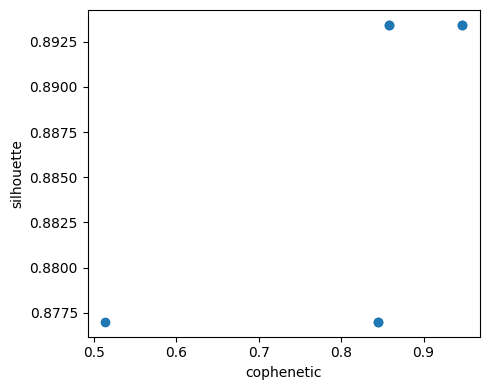
\includegraphics[width=0.8\columnwidth]{assets/1_coph_vs_silhouette.png}
	\caption{Cophenetic vs.\ silhouette for all configurations. Top-right indicates better fidelity and separation.}
	\label{fig:coph_vs_silhouette}
\end{figure}

Because \emph{single} linkage may form chaining clusters, we report two complementary views:
(i) the best-silhouette solution (\textbf{Single–Euclid, $k=3$}) and (ii) a robust alternative without single linkage
(\textbf{Average–Euclid, $k=4$}). The horizontal cut at the recorded equivalent threshold reproduces the same $k$ in the
dendrogram.

\begin{figure}[H]
	\centering
	% Replace with the dendrogram you want as the main figure
	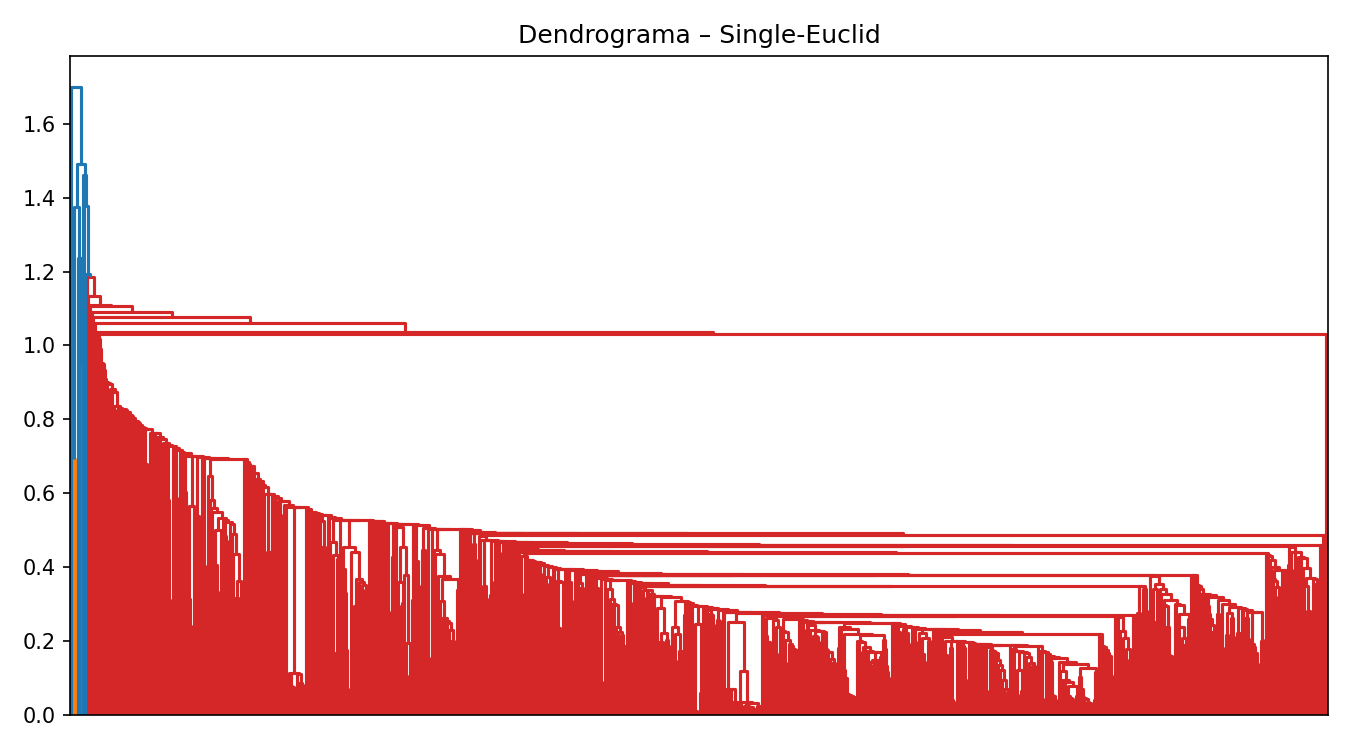
\includegraphics[width=0.8\columnwidth]{assets/4_dendogram_single.png}
	\caption{Dendrogram—Single–Euclidean. The horizontal cut at the equivalent threshold yields $k=3$.}
	\label{fig:dendro_single_euclid}
\end{figure}

Across configurations, a \emph{dominant} “catalog” cluster concentrates the bulk of models near global means, while
1–3 \emph{small} “elite” clusters group items with markedly higher \emph{downloads/likes/performance} and (on average)
lower \emph{size/CO\textsubscript{2}}. Variable importance from $z$–centroids is consistent: the most discriminative
feature is \textbf{downloads} (max $|z|\approx 5.39$), followed by \textbf{likes} ($\approx 2.03$), then
\emph{CO\textsubscript{2}} and \emph{performance} (moderate), with \emph{size} contributing less ($\approx 1.32$).

External validation against labels was limited, as expected (labels were not used to train the clustering):
ARI vs.\ \texttt{is\_fair} stayed near zero across settings; however, cluster–label contingency showed reasonable
purities (mean $\sim 0.73$–$0.90$ depending on the configuration), with \texttt{is\_fair=True} enriched in one of the small
clusters and scarce in the large catalog group.

% --- Suggested figures for the chosen config ---
\begin{figure}[H]
	\centering
	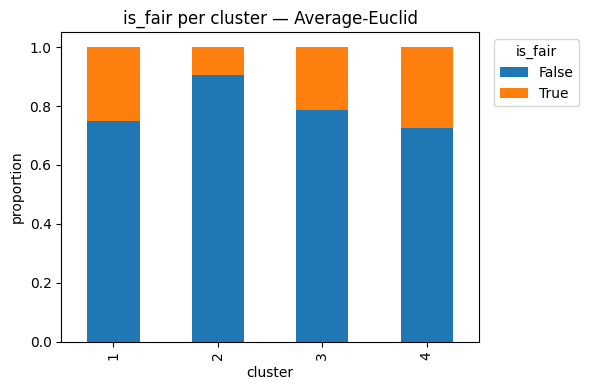
\includegraphics[width=0.8\columnwidth]{assets/3_is_fair_per_cluster.png}
	\caption{Stacked proportions of \texttt{is\_fair} per cluster (Average–Euclid, $k=4$).}
	\label{fig:isfair_stacked}
\end{figure}


\paragraph{Cluster profiles.}
Tables~\ref{tab:profile-a}–\ref{tab:profile-b} report \emph{original-unit} profiles (count/mean/median) for
\textit{performance\_score}, \textit{co2\_eq\_emissions}, \textit{likes}, \textit{downloads} and \textit{size}. For brevity,
we include the robust alternative (\emph{Average–Euclid, $k=4$}); the $z$–centroids and the $|z|$ ranking (downloads $\to$ likes)
appear in the Supplement.
\begin{table}[t]
	\centering
	\small
	\caption{Cluster profiles (original units): performance and CO$_2$}
	\label{tab:profile-a}
	\renewcommand{\arraystretch}{1.1}
	\begin{tabular}{l S[table-format=4.0] S[table-format=1.3] S[table-format=1.3]
			S[table-format=2.3] S[table-format=1.3]}
		\toprule
		& \multicolumn{3}{c}{\textbf{performance\_score}}
		& \multicolumn{2}{c}{\textbf{co2\_eq\_emissions}} \\
		\cmidrule(lr){2-4}\cmidrule(lr){5-6}
		\textbf{cluster} & \textbf{n} & \textbf{mean} & \textbf{median}
		& \textbf{mean} & \textbf{median} \\
		\midrule
		1 & 4    & 0.988 & 0.991 & 49.974 & 3.189 \\
		2 & 1029 & 0.727 & 0.822 & 71.382 & 2.749 \\
		\bottomrule
	\end{tabular}
\end{table}

\begin{table}[t]
	\centering
	\small
	\caption{Cluster profiles (original units): likes and downloads}
	\label{tab:profile-b}
	\renewcommand{\arraystretch}{1.1}
	\begin{tabular}{
			l
			S[table-format=4.0]        % n
			S[table-format=1.3]        % likes mean
			S[table-format=1.3]        % likes median
			S[table-format=6.2]        % downloads mean
			S[table-format=7.2]        % downloads median
		}
		\toprule
		& \multicolumn{3}{c}{\textbf{likes}}
		& \multicolumn{2}{c}{\textbf{downloads}} \\
		\cmidrule(lr){2-4}\cmidrule(lr){5-6}
		\textbf{cluster} & \textbf{n} & \textbf{mean} & \textbf{median}
		& \textbf{mean} & \textbf{median} \\
		\midrule
		1 & 4    & 2.250 & 0.500 & \num{104439.25} & \num{102572.50} \\
		2 & 1029 & 0.181 & 0.000 & \num{65.245}    & \num{5.00} \\
		\bottomrule
	\end{tabular}
\end{table}


\begin{table}[t]
	\centering
	\small
	\caption{Cluster profiles (original units): size ($\times 10^{8}$)}
	\label{tab:profile-c}
	\renewcommand{\arraystretch}{1.1}
	\begin{tabular}{l S[table-format=4.0] S[table-format=1.3] S[table-format=1.3]}
		\toprule
		\textbf{cluster} & \textbf{n} & \textbf{mean} & \textbf{median} \\
		\midrule
		1 & 4    & 2.649 & 2.654 \\
		2 & 1029 & 8.953 & 4.987 \\
		\bottomrule
	\end{tabular}
\end{table}

	\subsection{Limpieza de datos}
	En el anterior apartado se realizó un análisis general de los resultados y se encontró que las variables \texttt{size} y \texttt{size\_efficiency} poseen algunos datos nulos, cerca del 8\%, por lo tanto, es necesario aplicar una regresión, en la ruta del proyecto \texttt{notebooks/1\_2\_data\_cleaning.ipynb} se encuentra la implementación de la regresión y la limpieza de datos, se escogió la regresión, porque es la técnica que menos sesgos podría generar en el conjunto de datos, a diferencia de las otras formas de imputación.
	Luego de la imputación de variables, se limpiaron los valores infinitos, luego se realizó una estandarización, para realizar el análisis de varianza y de covarianza, en este punto se excluyen las variables categóricas

	\subsection{Análisis de covarianza y correlación}
	Para realizar el análisis de covarianza y correlación, lo primero es estandarizar los datos usando \texttt{StandardScaler} para presentarlos en la gráfica de manera más amigable, dado que las variables tienen una dispersión muy alta, a continuación se muestra la gráfica de correlación, ya que la de covarianza no permite ver las relaciones de manera tan clara


	Para interpretar las correlaciones, se toma de manera univariada las relaciones entre las variables del conjunto de datos
	\subsubsection{\texttt{co2\_eq\_emissions} vs. \texttt{likes}}

	Con una correlación de 0.99, esta es una correlación positiva extremadamente fuerte. Sugiere que los modelos de IA que tienen un mayor número de likes
	(\texttt{likes}) también tienden a tener una emisión de CO2 equivalente mucho más alta.
	\subsubsection{\texttt{co2\_eq\_emissions} vs. \texttt{size}}
	Con una correlación de 0.99, similar al caso anterior, existe una correlación positiva extremadamente fuerte. Esto implica que los modelos de IA más grandes en términos de tamaño (\texttt{size}) son los que emiten una mayor cantidad de CO2.

	\subsubsection{\texttt{co2\_eq\_emissions} vs. \texttt{downloads}}
	Con una correlación de 0.04, La correlación es prácticamente cero (muy débil). Esto indica que no hay una relación lineal significativa entre el número de descargas (\texttt{downloads}) y la cantidad de emisiones de CO2. Un modelo puede tener muchas descargas independientemente de su huella de carbono.

	\subsubsection{\texttt{co2\_eq\_emissions} vs. \texttt{size\_efficency}}
	Con una correlación de -0.01, La correlación es también cercana a cero. Esto sugiere que la eficiencia del tamaño (\texttt{size\_efficency}) no está linealmente relacionada con las emisiones de CO2. Es posible que esta variable no esté capturando la eficiencia en términos de emisiones, o que la relación sea no lineal.

	\subsection{Análisis de componentes principales (PCA) y factores principales (PFA)}
	Para este apartado, se excluyeron las variables cualitativas, y se conservó de las ejecuciones anteriores la base de datos de imputados, limpios y estandarizados, luego de estandarizar los datos, se le aplicó la función \texttt{fit\_transform} los detalles de la implementación se presentan en el notebook que se encuentra en la ruta: \texttt{3\_analisis\_factores.ipynb} del proyecto.
	\subsubsection{Análisis de componentes principales}
	El primer resultado que se encuentra es acerca de la varianza explicada, los resultados se encuentran consolidados en la siguiente tabla:

	\begin{table}[H]
		\centering
		\caption{Resultados del Análisis de Componentes Principales}
		\begin{tabular}{l c c c}
			\toprule
			Componente & Valor propio & Varianza Explicada & Varianza Acumulada \\
			\midrule
			PC1 & 2.989 & 59.74\% & 59.74\% \\
			PC2 & 1.012 & 20.23\% & 79.97\% \\
			PC3 & 0.988 & 19.75\% & 99.72\% \\
			PC4 & 0.010 & 0.21\%  & 99.93\% \\
			PC5 & 0.003 & 0.07\% & 100.00\% \\
			\bottomrule
		\end{tabular}
		\label{tab:pca_results}
	\end{table}
	\subsubsection{Interpretación de los resultados}
	\begin{itemize}
		\item \textbf{Componente 1}: Con un valor propio de \texttt{2.989}, este componente es el más importante. Explica casi el 60\% de la varianza total de los datos por sí solo. Esto significa que la mayor parte de la información está concentrada en esta primera dimensión.
		\item \textbf{Componente 2}: Explica un \texttt{20.23\%} de la varianza. Al combinarlo con el Componente 1, ambos componentes juntos explican casi el \texttt{80\%} de la varianza acumulada.
		\item \textbf{Componente 3}: Este componente explica casi un 20\% de la varianza. Al incluirlo, la varianza acumulada asciende al \texttt{99.72\%}.
		\item \textbf{Componentes 4 y 5}: Estos componentes tienen valores propios muy pequeños y explican una varianza insignificante (menos del 1\% entre ambos).
	\end{itemize}
	\subsubsection{Selección de componentes}
	Para decidir cuántos componentes conservar, se aplicó el criterio de  Kaiser, que sugiere mantener los componentes con un valor propio mayor a 1.
	Según este criterio, se deberías considerar conservar solo los dos primeros componentes principales, ya que sus valores propios son \texttt{2.989} y \texttt{1.012}.
	Estos dos componentes juntos resumen el \texttt{79.97\%} de la varianza de tus datos, conservarlos permite reducir la dimensionalidad del conjunto de datos de cinco variables a solo dos, perdiendo muy poca información esencial.
	A continuación, se presenta la matriz de cargas factoriales para los componentes principales. Cada valor indica la correlación de la variable original con el componente correspondiente.

	\begin{table}[H]
		\centering
		\caption{Resultados del Análisis de Componentes Principales}
		\begin{tabular}{l c c c}
			\toprule
			Variable Original & Carga en PC1 & Carga en PC2 \\
			\midrule
			\texttt{co2\_eq\_emissions} & 0.577 & 0.047 \\
			\texttt{downloads} & 0.033 & -0.695 \\
			\texttt{likes} & -0.031 & 0.715 \\
			\texttt{size} & -0.126 & 0.052 \\
			\texttt{size\_efficency} & 0.805 & 0.031 \\
			\bottomrule
		\end{tabular}
		\label{tab:pca_results}
	\end{table}


	\subsubsection{Interpretación de los Componentes Principales Clave}
	\begin{itemize}
		\item \textbf{Componente 1 (PC1)}: Este componente, que explica la mayor parte de la varianza del conjunto de datos, está fuertemente asociado con las variables 4 y 0. Ambas contribuyen de manera positiva a este componente, sugiriendo que el PC1 captura un factor común de estas dos variables.
		\item \textbf{Componente 2 (PC2)}: Este componente representa un contraste entre la variable 2 y la variable 1. La alta carga positiva de la variable 2 y la alta carga negativa de la variable 1 indican que el PC2 describe una relación inversamente proporcional entre ellas."
	\end{itemize}

	\begin{itemize}
		\item \textbf{Varianza en el PC1}: La mayoría de los puntos se agrupan cerca de la coordenada 0 en el eje horizontal, con la notable excepción de un punto que se encuentra muy alejado, alrededor de PC1 = 60. Este punto atípico (o outlier) es una observación con un valor extremadamente alto en el primer componente principal. La gran dispersión a lo largo del eje horizontal refuerza lo que vimos en el análisis de los valores propios: el PC1 captura la mayor parte de la varianza en tus datos.
		\item \textbf{Varianza en el PC2}: En el eje vertical (PC2), los puntos también están bastante concentrados cerca de la coordenada 0, aunque hay una mayor dispersión vertical en este grupo principal. Hay un par de puntos que se alejan del grupo, pero la variabilidad es considerablemente menor en comparación con el PC1. Esto confirma que el PC2 explica menos varianza que el PC1.
		\item \textbf{Presencia de un Outlier}:  La observación aislada en la esquina inferior derecha es un caso extremo. Este punto tiene un valor muy alto en el PC1 y un valor moderadamente bajo en el PC2. Es probable que esta observación represente un modelo de IA con características extremas en las variables originales que más contribuyen al PC1 (por ejemplo, un tamaño o una emisión de CO2 excepcionalmente grandes).
	\end{itemize}

	\subsubsection{Análsis de factores principales (PFA)}
	Para el Análisis Factorial de Principales Componentes (PFA), los números que ha obtenido son los valores propios (eigenvalues) de los factores. A diferencia del PCA, donde los valores propios explican la varianza total de los datos, en el PFA estos valores explican solo la varianza común (o compartida) entre las variables, lo cual es la varianza que puede atribuirse a factores subyacentes.
	La interpretación de los resultados se presenta a continuación en la siguiente tabla:
	\begin{table}[H]
		\centering
		\caption{Interpretación de Factores Principales}
		\begin{tabular}{l c c c}
			\toprule
			Factor & Valor propio & \% de Varianza Común Explicada & \% Acumulado	 \\
			\midrule
			\texttt{F1} & 2.987 &    74.49\% & 74.49\%  \\
			\texttt{F2} & 1.012 &    25.26\% & 99.75\%  \\
			\texttt{F3} & 0.988 &    0.22\%  & 99.97\%   \\
			\texttt{F4} & 0.010 &    0.03\%  & 100.00\%   \\
			\texttt{F5} & 0.003 &    0.00\%  & 100.00\%  \\
			\bottomrule
		\end{tabular}
		\label{tab:pca_results}
	\end{table}
	\subsubsection{Interpretación de factores (PFA)}
	\begin{itemize}
		\item \textbf{Factor 1 (Valor Propio: 2.987)}: Este factor captura la mayor parte de la varianza compartida, explicando un notable 74.49\% de ella por sí solo. Es, con diferencia, el factor más importante.
		\item \textbf{Factor 2 (Valor Propio: 1.012)}: Este factor también es muy significativo, ya que explica otro 25.26\% de la varianza común. Al combinar el Factor 1 y el Factor 2, se explica casi el 99.75\% de toda la variabilidad compartida de tu conjunto de datos.
		\item \textbf{Factores Restantes (3, 4 y 5)}: Los valores propios de estos factores son muy bajos, lo que indica que explican una cantidad insignificante de la varianza común
	\end{itemize}
	Para determinar cuantos factores retener, se usa el criterio de kaiser, el detalle de la implementación puede verse en la ruta: \texttt{notebooks/3\_analisis\_factores.ipynb}
	\subsubsection{Análisis de cargas factoriales}
	El Factor 1 es el más significativo, tal como lo vimos en el análisis de los valores propios. Las variables con las cargas más altas en este factor son:
	\begin{itemize}
		\item \texttt{co2\_eq\_emissions}: \texttt{0.999200}
		\item \texttt{likes}: \texttt{0.995705}
		\item \texttt{size}: \texttt{0.993753}
	\end{itemize}
	Estos valores son extremadamente altos, lo que significa que el Factor 1 es, en esencia, un resumen de estas tres variables. Todas ellas tienen una correlación positiva muy fuerte con el factor, lo que sugiere que los modelos con un gran tamaño y un alto número de likes tienden a tener una alta emisión de CO2. Este factor puede ser interpretado como un factor de "Complejidad y Popularidad del Modelo" que está directamente relacionado con la huella de carbono.
	Las variables \texttt{downloads} y \texttt{size\_efficency} tienen cargas muy bajas en el Factor 1, lo que indica que no contribuyen significativamente a este factor latente.
	El Factor 2 explica la varianza común restante. La variable con la carga más alta en este factor es \texttt{downloads}: \texttt{0.718192}. Esto sugiere que el Factor 2 está definido principalmente por el número de descargas. Las otras variables tienen cargas muy bajas, lo que indica que no están fuertemente correlacionadas con este factor. Por lo tanto, el Factor 2 puede ser interpretado como un factor de "Alcance o Adopción del Modelo", que es conceptualmente distinto del primer factor.
	Los resultados confirman que las variables de emisiones de CO2, likes y tamaño están altamente correlacionadas y se agrupan en el mismo constructo subyacente, mientras que las descargas representan un concepto separado el conjunto datos.

	El gráfico de sedimento confirma visualmente lo que los valores numéricos indicaban: los Factores 1 y 2 son los más significativos y los únicos que vale la pena conservar para el análisis. Los factores 3, 4 y 5 tienen valores propios muy bajos, lo que significa que explican una cantidad trivial de varianza y pueden ser descartados.
	A continuación se presentan los biplots de los métodos PCA y PFA


	\subsubsection{Interpretación de Biplots}
	\textbf{Para el biplot de factores principales}: \textbf{Factor1 popularidad y tamaño:} Este factor, representado por el eje horizontal, está fuertemente correlacionado con las variables likes, \texttt{co2\_emissions} y \texttt{size}. Las aplicaciones con valores altos en este factor tienden a ser más populares, con una mayor cantidad de 'me gusta', un tamaño de archivo más grande y, posiblemente, un mayor impacto ambiental.
	\textbf{Factor 2} Capacidad de Descarga: este factor, representado por el eje vertical, se relaciona principalmente con la variable downloads. Indica que las aplicaciones con altas puntuaciones en este factor son las que tienen un alto número de descargas, independientemente de su popularidad o tamaño.
	La mayoría de las observaciones se agrupan en el centro, lo que sugiere que la mayoría de las aplicaciones tienen características promedio. Sin embargo, se pueden identificar dos grupos distintos de aplicaciones:
	\begin{itemize}
		\item Las que se caracterizan por una alta popularidad y tamaño (Factor 1).
		\item Las que se distinguen por un alto número de descargas (Factor 2).
	\end{itemize}
	La variable size\_efficiency muestra una correlación muy baja con ambos factores, lo que indica que no es un buen predictor de la popularidad, el tamaño o las descargas de una aplicación.
	En cuanto al biplot de análisis de componentes principales. El PC1, que explica la mayor parte de la varianza en los datos, establece un contraste directo entre likes y downloads. Esto indica una fuerte correlación negativa: las aplicaciones con un alto número de "me gusta" tienden a tener pocas descargas, mientras que aquellas con muchas descargas reciben menos "me gusta". Esto podría sugerir dos estrategias distintas de éxito. Además, el PC2 no es un factor dominante, ya que las variables size, size\_efficiency y co2\_eq\_emissions tienen una baja correlación con él. Esto significa que estas variables no aportan valor para explicar la principal variabilidad del conjunto de datos. y En síntesis:
	El biplot revela que la varianza de los datos se explica principalmente por una sola dimensión: el equilibrio entre la popularidad social y el volumen de descargas. Las otras variables tienen un impacto mínimo en la forma en que tus datos se agrupan.

	\section{Conclusión}
	\label{sec:conclusion}
	El análisis comparativo de las técnicas multivariadas aplicadas al conjunto de datos, específicamente el Análisis de Componentes Principales (PCA) y el Análisis de Factores Principales (PFA), ha revelado información crucial sobre la estructura subyacente de las variables.

	\subsection{Justificación del Método Seleccionado}
	El Análisis de Factores Principales (PFA) se identifica como el método más apropiado para este estudio. Aunque el PCA logró identificar una dimensión de varianza predominante, su principal objetivo es la reducción de dimensionalidad y no la interpretación de constructos latentes. En contraste, el PFA, diseñado para tal fin, proporcionó un modelo más robusto y conceptualmente interpretable.

	\subsection{Hallazgos encontrados}
	El modelo de PFA extrajo satisfactoriamente dos factores latentes que explican las interrelaciones observadas entre las variables.  Estos factores se interpretan de la siguiente manera:

	Factor 1: Popularidad y Escala. Este factor se correlaciona fuertemente con las variables likes, co2\_emissions y size. Dicho factor representa un constructo de éxito que agrupa atributos de popularidad y tamaño.

	Factor 2: Capacidad de Adquisición. Este factor está casi exclusivamente definido por la variable downloads. Su independencia del Factor 1 sugiere que la capacidad de una aplicación para ser descargada es una dimensión distinta y no redundante del éxito.

	\subsection{Implicaciones}
	Los resultados demuestran que el comportamiento de las aplicaciones no se puede explicar adecuadamente por una sola dimensión, sino que está influenciado por al menos dos constructos subyacentes. La identificación de estos factores permite una comprensión más profunda de la dinámica del mercado y proporciona una base sólida para la toma de decisiones estratégicas, orientadas a optimizar el rendimiento en cada una de estas dimensiones independientes.

	\subsection{Conclusión final}
	Aunque el conjunto de datos es funcional para un análisis exploratorio, su limitada granularidad y la ausencia de estandarización en las métricas de evaluación impiden un análisis riguroso de la huella de carbono. La variabilidad en el hardware utilizado, la ubicación geográfica de los centros de datos y la falta de consistencia en los informes de consumo energético y emisiones de CO2 representan obstáculos significativos para identificar con certeza las variables más influyentes.
	Estos factores comprometen la capacidad de extraer conclusiones definitivas sobre la relación entre las configuraciones de los modelos de inteligencia artificial y su impacto ambiental. Por lo tanto, se enfatiza la necesidad de futuros estudios que se beneficien de conjuntos de datos más detallados, actualizados y estandarizados. Un enfoque más riguroso en la recopilación de datos permitirá una comprensión más profunda del impacto ambiental de la IA y facilitará el desarrollo de prácticas más sostenibles en la industria.

	\bibliographystyle{IEEEtran}

	\bibliography{mybibfile}
\end{document}